\documentclass{agony}
\title{SPH4U: Dynamics Assignment}

\begin{document}
\thispagestyle{firstpage}
\textbf{\thetitle}

\begin{prob}
	Two heavy boxes, $m_{1}$ and $m_{2}$, lie stationary on different inclines, as shown.
	A rope runs over a pulley and connects the boxes.
	Mass 1, $m_{1}$ is 380 kg. Assuming that each incline is frictionless and the system is in equilibrium, answer the
	following:

	\begin{enumerate}[(a)]
		\item \textbf{Draw FBD(s).}\\
		      \begin{minipage}[t]{.5\textwidth}
			      \underline{$m_{1}$ FBD:}
			      \tikzset{every picture/.style={line width=0.75pt}} %set default line width to 0.75pt        

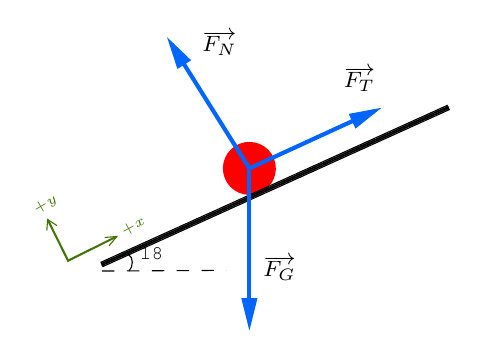
\begin{tikzpicture}[x=0.75pt,y=0.75pt,yscale=-1,xscale=1]
	%uncomment if require: \path (0,300); %set diagram left start at 0, and has height of 300

	%Shape: Ellipse [id:dp1428949648769431] 
	\draw  [color={rgb, 255:red, 255; green, 0; blue, 0 }  ,draw opacity=1 ][fill={rgb, 255:red, 254; green, 0; blue, 0 }  ,fill opacity=1 ] (149.04,183.11) .. controls (147.8,176.33) and (152.3,169.83) .. (159.09,168.59) .. controls (165.87,167.35) and (172.38,171.85) .. (173.61,178.64) .. controls (174.85,185.42) and (170.35,191.93) .. (163.56,193.16) .. controls (156.78,194.4) and (150.28,189.9) .. (149.04,183.11) -- cycle ;
	%Shape: Rectangle [id:dp48287918810377195] 
	\draw   (89.84,226.09) -- (256.64,150.53) -- (256.96,151.22) -- (90.15,226.78) -- cycle ;
	%Shape: Rectangle [id:dp005233673921997584] 
	\draw   (90.15,226.78) -- (256.96,151.22) -- (257.27,151.91) -- (90.46,227.47) -- cycle ;
	%Shape: Rectangle [id:dp9526931686132831] 
	\draw   (90.46,227.47) -- (257.27,151.91) -- (257.58,152.6) -- (90.77,228.16) -- cycle ;

	%Straight Lines [id:da8350690671631047] 
	\draw [color={rgb, 255:red, 1; green, 101; blue, 255 }  ,draw opacity=1 ][line width=1.5]    (161.33,180.88) -- (161.33,255.01) ;
	\draw [shift={(161.33,259.01)}, rotate = 270] [fill={rgb, 255:red, 1; green, 101; blue, 255 }  ,fill opacity=1 ][line width=0.08]  [draw opacity=0] (15.6,-3.9) -- (0,0) -- (15.6,3.9) -- cycle    ;
	%Straight Lines [id:da1062981577052522] 
	\draw [color={rgb, 255:red, 1; green, 101; blue, 255 }  ,draw opacity=1 ][line width=1.5]    (161.33,180.88) -- (123.79,121.05) ;
	\draw [shift={(121.67,117.67)}, rotate = 57.89] [fill={rgb, 255:red, 1; green, 101; blue, 255 }  ,fill opacity=1 ][line width=0.08]  [draw opacity=0] (15.6,-3.9) -- (0,0) -- (15.6,3.9) -- cycle    ;
	%Straight Lines [id:da21972886949175963] 
	\draw [color={rgb, 255:red, 1; green, 101; blue, 255 }  ,draw opacity=1 ][line width=1.5]    (161.33,180.88) -- (221.36,153.33) ;
	\draw [shift={(225,151.67)}, rotate = 155.36] [fill={rgb, 255:red, 1; green, 101; blue, 255 }  ,fill opacity=1 ][line width=0.08]  [draw opacity=0] (15.6,-3.9) -- (0,0) -- (15.6,3.9) -- cycle    ;
	%Shape: Right Angle [id:dp7929492774408056] 
	\draw  [color={rgb, 255:red, 65; green, 117; blue, 5 }  ,draw opacity=1 ][line width=0.75]  (97.31,213.73) -- (73.99,225.35) -- (64.15,205.57) ;
	\draw  [color={rgb, 255:red, 65; green, 117; blue, 5 }  ,draw opacity=1 ] (63.75,210.84) -- (64.11,205.52) -- (68.6,208.42) ;
	\draw  [color={rgb, 255:red, 65; green, 117; blue, 5 }  ,draw opacity=1 ] (91.56,214.16) -- (97.45,213.7) -- (93.7,218.23) ;

	%Curve Lines [id:da5437896212575373] 
	\draw    (103,222.33) .. controls (105.67,223.67) and (105.33,228.33) .. (103.33,230.33) ;
	%Straight Lines [id:da9621621519167294] 
	\draw  [dash pattern={on 4.5pt off 4.5pt}]  (90.33,230.33) -- (150.33,230) ;

	% Text Node
	\draw (166.85,221.91) node [anchor=north west][inner sep=0.75pt]  [font=\footnotesize] [align=left] {$\displaystyle \overrightarrow{F_{G}}$};
	% Text Node
	\draw (205.56,130.62) node [anchor=north west][inner sep=0.75pt]  [font=\footnotesize] [align=left] {$\displaystyle \overrightarrow{F_{T}}$};
	% Text Node
	\draw (137.43,113.35) node [anchor=north west][inner sep=0.75pt]  [font=\footnotesize,color={rgb, 255:red, 0; green, 0; blue, 0 }  ,opacity=1 ] [align=left] {$\displaystyle \overrightarrow{F_{N}}$};
	% Text Node
	\draw (107.33,218) node [anchor=north west][inner sep=0.75pt]  [font=\scriptsize] [align=left] {{\fontfamily{pcr}\selectfont 18}$\displaystyle \degree $};
	% Text Node
	\draw (97.11,208.66) node [anchor=north west][inner sep=0.75pt]  [font=\tiny,color={rgb, 255:red, 65; green, 117; blue, 5 }  ,opacity=1 ,rotate=-331] [align=left] {$\displaystyle +x$};
	% Text Node
	\draw (54.78,198.23) node [anchor=north west][inner sep=0.75pt]  [font=\tiny,color={rgb, 255:red, 65; green, 117; blue, 5 }  ,opacity=1 ,rotate=-329.58] [align=left] {$\displaystyle +y$};


\end{tikzpicture}
		      \end{minipage}%
		      \begin{minipage}[t]{.5\textwidth}
			      \underline{$m_{2}$ FBD:}
			      

\tikzset{every picture/.style={line width=0.75pt}} %set default line width to 0.75pt        

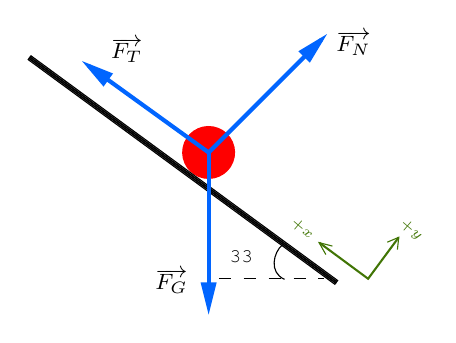
\begin{tikzpicture}[x=0.75pt,y=0.75pt,yscale=-1,xscale=1]
	%uncomment if require: \path (0,300); %set diagram left start at 0, and has height of 300

	%Shape: Ellipse [id:dp1428949648769431] 
	\draw  [color={rgb, 255:red, 255; green, 0; blue, 0 }  ,draw opacity=1 ][fill={rgb, 255:red, 254; green, 0; blue, 0 }  ,fill opacity=1 ] (198.05,181.45) .. controls (199.28,174.66) and (194.78,168.16) .. (188,166.92) .. controls (181.21,165.69) and (174.71,170.19) .. (173.47,176.97) .. controls (172.24,183.76) and (176.74,190.26) .. (183.52,191.5) .. controls (190.31,192.73) and (196.81,188.23) .. (198.05,181.45) -- cycle ;
	%Shape: Rectangle [id:dp48287918810377195] 
	\draw   (247.91,240.87) -- (100.19,132.64) -- (99.74,133.25) -- (247.46,241.49) -- cycle ;
	%Shape: Rectangle [id:dp005233673921997584] 
	\draw   (247.46,241.49) -- (99.74,133.25) -- (99.29,133.87) -- (247.01,242.1) -- cycle ;
	%Shape: Rectangle [id:dp9526931686132831] 
	\draw   (247.01,242.1) -- (99.29,133.87) -- (98.85,134.48) -- (246.56,242.71) -- cycle ;

	%Straight Lines [id:da8350690671631047] 
	\draw [color={rgb, 255:red, 1; green, 101; blue, 255 }  ,draw opacity=1 ][line width=1.5]    (185.76,179.21) -- (185.76,253.35) ;
	\draw [shift={(185.76,257.35)}, rotate = 270] [fill={rgb, 255:red, 1; green, 101; blue, 255 }  ,fill opacity=1 ][line width=0.08]  [draw opacity=0] (15.6,-3.9) -- (0,0) -- (15.6,3.9) -- cycle    ;
	%Straight Lines [id:da1062981577052522] 
	\draw [color={rgb, 255:red, 1; green, 101; blue, 255 }  ,draw opacity=1 ][line width=1.5]    (185.76,179.21) -- (239.99,124.98) ;
	\draw [shift={(242.82,122.15)}, rotate = 135] [fill={rgb, 255:red, 1; green, 101; blue, 255 }  ,fill opacity=1 ][line width=0.08]  [draw opacity=0] (15.6,-3.9) -- (0,0) -- (15.6,3.9) -- cycle    ;
	%Straight Lines [id:da21972886949175963] 
	\draw [color={rgb, 255:red, 1; green, 101; blue, 255 }  ,draw opacity=1 ][line width=1.5]    (185.76,179.21) -- (128.01,137.53) ;
	\draw [shift={(124.77,135.19)}, rotate = 35.82] [fill={rgb, 255:red, 1; green, 101; blue, 255 }  ,fill opacity=1 ][line width=0.08]  [draw opacity=0] (15.6,-3.9) -- (0,0) -- (15.6,3.9) -- cycle    ;
	%Shape: Right Angle [id:dp7929492774408056] 
	\draw  [color={rgb, 255:red, 65; green, 117; blue, 5 }  ,draw opacity=1 ][line width=0.75]  (239.14,222.71) -- (262.61,240.05) -- (277.31,220.15) ;
	\draw  [color={rgb, 255:red, 65; green, 117; blue, 5 }  ,draw opacity=1 ] (276.72,226.04) -- (277.35,220.09) -- (271.84,222.43) ;
	\draw  [color={rgb, 255:red, 65; green, 117; blue, 5 }  ,draw opacity=1 ] (245.39,224.3) -- (238.99,222.65) -- (242.24,228.38) ;

	%Curve Lines [id:da5437896212575373] 
	\draw    (221.33,223.67) .. controls (217,227.33) and (214.67,237) .. (222.33,240.33) ;
	%Straight Lines [id:da5100408990791785] 
	\draw  [dash pattern={on 4.5pt off 4.5pt}]  (190.67,240) -- (241.33,240) ;

	% Text Node
	\draw (158.85,233.91) node [anchor=north west][inner sep=0.75pt]  [font=\footnotesize] [align=left] {$\displaystyle \overrightarrow{F_{G}}$};
	% Text Node
	\draw (137.56,122.62) node [anchor=north west][inner sep=0.75pt]  [font=\footnotesize] [align=left] {$\displaystyle \overrightarrow{F_{T}}$};
	% Text Node
	\draw (246.09,119.35) node [anchor=north west][inner sep=0.75pt]  [font=\footnotesize,color={rgb, 255:red, 0; green, 0; blue, 0 }  ,opacity=1 ] [align=left] {$\displaystyle \overrightarrow{F_{N}}$};
	% Text Node
	\draw (194.67,225) node [anchor=north west][inner sep=0.75pt]  [font=\scriptsize] [align=left] {{\fontfamily{pcr}\selectfont 33}$\displaystyle \degree $};
	% Text Node
	\draw (227.99,208.32) node [anchor=north west][inner sep=0.75pt]  [font=\tiny,color={rgb, 255:red, 65; green, 117; blue, 5 }  ,opacity=1 ,rotate=-40.39] [align=left] {$\displaystyle +x$};
	% Text Node
	\draw (280.67,208.71) node [anchor=north west][inner sep=0.75pt]  [font=\tiny,color={rgb, 255:red, 65; green, 117; blue, 5 }  ,opacity=1 ,rotate=-40.39] [align=left] {$\displaystyle +y$};


\end{tikzpicture}
		      \end{minipage}

		\item \textbf{Find the magnitude of the tension in the cable.}\\
		      \begin{solution}
			      \vec{F_{net_{1x}}}            & = 0                                                              \\
			      0                             & = \vec{F_{g}} \sin 18\degree + \left\lvert F_{T}\right\rvert \\
			      0                             & = m_{1}g \sin 18 \degree + \left\lvert F_{T}\right\rvert         \\
			      0                             & = 380(-9.8) \sin 18 \degree + \left\lvert F_{T}\right\rvert      \\
			      \left\lvert F_{T}\right\rvert & = 1150.78\text{N}                                                \\
			      \left\lvert F_{T}\right\rvert & = 1200~\text{N}                                                  \\
		      \end{solution}
		      $\therefore$ The magnitude of tension in the string is 1200 N.

		\item \textbf{Calculate the mass of \bm{$m_{2}$} needed to keep the system in equilibrium.}

		      \begin{solution}
			      F_{net_{2x}} & = 0                                         \\
			      0            & = \vec{F_{g}} \sin 33 \degree + 1150.78 \\
			      m_{2}        & = \frac{-1150.78}{-9.8\sin 33 \degree}      \\
			      m_{2}        & = 215.6\text{kg}                            \\
			      m_{2}        & = 220~\text{kg}
		      \end{solution}
		      $\therefore$ The mass of the second box ($m_{2}$) is 220 kg.
	\end{enumerate}
\end{prob}

\begin{prob}
	A girl applies a 140 N force to a 35.0 kg bale of hay at an angle of 28\textdegree~above the horizontal.
	The force of friction acting on the bale is 55 N.
	\begin{enumerate}[(a)]
		\item \textbf{What will be the horizontal acceleration of the bale?}
		      \begin{solution}
			      \vec{F_{net_{x}}} & = \vec{F_{a_{x}}} - \vec{F_{f}} & \vec{F_{net_{x}}} & = m\vec{a}                                 \\
			      & = 140 \cos 28\degree - 55       &\tab 66.81             & = 35\vec{a}                                \\
			      & = 66.81~\text{N[right]}         &\tab \vec{a}           & = 1.96\text{m/s\textsuperscript{2}[right]} \\
			      &                                 &\tab \vec{a}           & = 2.0~\text{m/s\textsuperscript{2}[right]}
		      \end{solution}
		      $\therefore$ The horizontal acceleration is 2.0 m/s\textsuperscript{2}[right]
		      \newpage
		\item \textbf{What is the coefficient of friction between the bale and the ground?}
		      \begin{solution}
			      \vec{F_{f}} &= \mu_{f}\vec{F_{N}}\\
			      55 &= \mu_{f}(\vec{F_{g}} - \vec{F_{a_{y}}})\\
			      \mu_{f} &= \frac{55}{35\times 9.8-140\sin 28\degree}\\
			      \mu_{f} &= 0.198
		      \end{solution}
		      $\therefore$ The coefficient of friction between the bale and ground is 0.20.
	\end{enumerate}

\end{prob}

\begin{prob}
	A 15kg box is pushed up a 35\textdegree~ramp.
	A force of 110 N exists between the box and the ramp.
	\begin{enumerate}[(a)]
		\item \textbf{Draw an FBD showing a tilted coordinate system (label positive x-direction)}\\
		      \begin{center}
			      \tikzset{every picture/.style={line width=0.75pt}} %set default line width to 0.75pt        

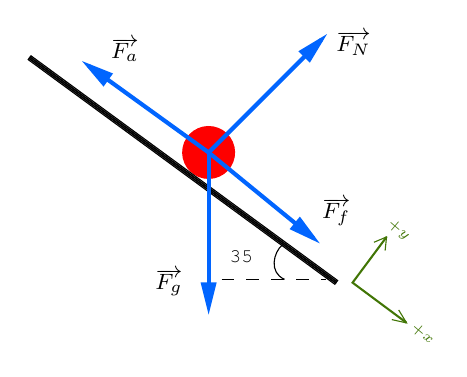
\begin{tikzpicture}[x=0.75pt,y=0.75pt,yscale=-1,xscale=1]
	%uncomment if require: \path (0,300); %set diagram left start at 0, and has height of 300

	%Shape: Ellipse [id:dp1428949648769431] 
	\draw  [color={rgb, 255:red, 255; green, 0; blue, 0 }  ,draw opacity=1 ][fill={rgb, 255:red, 254; green, 0; blue, 0 }  ,fill opacity=1 ] (198.05,181.45) .. controls (199.28,174.66) and (194.78,168.16) .. (188,166.92) .. controls (181.21,165.69) and (174.71,170.19) .. (173.47,176.97) .. controls (172.24,183.76) and (176.74,190.26) .. (183.52,191.5) .. controls (190.31,192.73) and (196.81,188.23) .. (198.05,181.45) -- cycle ;
	%Shape: Rectangle [id:dp48287918810377195] 
	\draw   (247.91,240.87) -- (100.19,132.64) -- (99.74,133.25) -- (247.46,241.49) -- cycle ;
	%Shape: Rectangle [id:dp005233673921997584] 
	\draw   (247.46,241.49) -- (99.74,133.25) -- (99.29,133.87) -- (247.01,242.1) -- cycle ;
	%Shape: Rectangle [id:dp9526931686132831] 
	\draw   (247.01,242.1) -- (99.29,133.87) -- (98.85,134.48) -- (246.56,242.71) -- cycle ;

	%Straight Lines [id:da8350690671631047] 
	\draw [color={rgb, 255:red, 1; green, 101; blue, 255 }  ,draw opacity=1 ][line width=1.5]    (185.76,179.21) -- (185.76,253.35) ;
	\draw [shift={(185.76,257.35)}, rotate = 270] [fill={rgb, 255:red, 1; green, 101; blue, 255 }  ,fill opacity=1 ][line width=0.08]  [draw opacity=0] (15.6,-3.9) -- (0,0) -- (15.6,3.9) -- cycle    ;
	%Straight Lines [id:da1062981577052522] 
	\draw [color={rgb, 255:red, 1; green, 101; blue, 255 }  ,draw opacity=1 ][line width=1.5]    (185.76,179.21) -- (239.99,124.98) ;
	\draw [shift={(242.82,122.15)}, rotate = 135] [fill={rgb, 255:red, 1; green, 101; blue, 255 }  ,fill opacity=1 ][line width=0.08]  [draw opacity=0] (15.6,-3.9) -- (0,0) -- (15.6,3.9) -- cycle    ;
	%Straight Lines [id:da21972886949175963] 
	\draw [color={rgb, 255:red, 1; green, 101; blue, 255 }  ,draw opacity=1 ][line width=1.5]    (185.76,179.21) -- (128.01,137.53) ;
	\draw [shift={(124.77,135.19)}, rotate = 35.82] [fill={rgb, 255:red, 1; green, 101; blue, 255 }  ,fill opacity=1 ][line width=0.08]  [draw opacity=0] (15.6,-3.9) -- (0,0) -- (15.6,3.9) -- cycle    ;
	%Shape: Right Angle [id:dp7929492774408056] 
	\draw  [color={rgb, 255:red, 65; green, 117; blue, 5 }  ,draw opacity=1 ][line width=0.75]  (281.02,261.19) -- (255.11,241.93) -- (271.45,219.97) ;
	\draw  [color={rgb, 255:red, 65; green, 117; blue, 5 }  ,draw opacity=1 ] (265.4,222.48) -- (271.49,219.9) -- (270.8,226.48) ;
	\draw  [color={rgb, 255:red, 65; green, 117; blue, 5 }  ,draw opacity=1 ] (277.33,255.08) -- (281.14,261.33) -- (274.03,259.73) ;

	%Straight Lines [id:da0016552996956802346] 
	\draw [color={rgb, 255:red, 1; green, 101; blue, 255 }  ,draw opacity=1 ][line width=1.5]    (185.76,179.21) -- (236.24,220.47) ;
	\draw [shift={(239.33,223)}, rotate = 219.26] [fill={rgb, 255:red, 1; green, 101; blue, 255 }  ,fill opacity=1 ][line width=0.08]  [draw opacity=0] (15.6,-3.9) -- (0,0) -- (15.6,3.9) -- cycle    ;
	%Curve Lines [id:da5437896212575373] 
	\draw    (221.33,223.67) .. controls (217,227.33) and (214.67,237) .. (222.33,240.33) ;
	%Straight Lines [id:da6898758265813036] 
	\draw  [dash pattern={on 4.5pt off 4.5pt}]  (192,240.33) -- (242.33,240.33) ;

	% Text Node
	\draw (158.85,233.91) node [anchor=north west][inner sep=0.75pt]  [font=\footnotesize] [align=left] {$\displaystyle \overrightarrow{F_{g}}$};
	% Text Node
	\draw (137.56,122.62) node [anchor=north west][inner sep=0.75pt]  [font=\footnotesize] [align=left] {$\displaystyle \overrightarrow{F_{a}}$};
	% Text Node
	\draw (246.09,119.35) node [anchor=north west][inner sep=0.75pt]  [font=\footnotesize,color={rgb, 255:red, 0; green, 0; blue, 0 }  ,opacity=1 ] [align=left] {$\displaystyle \overrightarrow{F_{N}}$};
	% Text Node
	\draw (239.23,199.96) node [anchor=north west][inner sep=0.75pt]  [font=\footnotesize] [align=left] {$\displaystyle \overrightarrow{F_{f}}$};
	% Text Node
	\draw (194.67,225) node [anchor=north west][inner sep=0.75pt]  [font=\scriptsize] [align=left] {{\fontfamily{pcr}\selectfont 35}$\displaystyle \degree $};
	% Text Node
	\draw (285.99,258.65) node [anchor=north west][inner sep=0.75pt]  [font=\tiny,color={rgb, 255:red, 65; green, 117; blue, 5 }  ,opacity=1 ,rotate=-40.39] [align=left] {$\displaystyle +x$};
	% Text Node
	\draw (274.67,208.71) node [anchor=north west][inner sep=0.75pt]  [font=\tiny,color={rgb, 255:red, 65; green, 117; blue, 5 }  ,opacity=1 ,rotate=-40.39] [align=left] {$\displaystyle +y$};


\end{tikzpicture}
		      \end{center}
		\item \textbf{What minimum force, \bm{$F$}, would be  necessary to move the box up the ramp at a constant speed?}
		      \begin{solution}
			      \vec{F_{net_{x}}} &= \vec{F_{a}} + \vec{F_{g_{x}}} + \vec{F_{f}}\\
			      0 &= \vec{F_{a}} + 15(-9.8)\sin 35\degree - 110\\
			      0 &= \vec{F_{a}} - 194.31\\
			      \vec{F_{a}} &= 194.31~\text{N}
		      \end{solution}
		      $\therefore$ Since constant speed implies no acceleration ($\vec{F_{net}}=0$), the force required to move the box at constant speed must also result in 0 net force, meaning the minimum force required is 190 N.
	\end{enumerate}
\end{prob}

\begin{prob}
	The apparatus shown in the diagram consists of a box of books connected by a string to a hanger plate loaded with masses.
	The mass, $m_{1}$, is for the box and books and the mass, $m_{2}$ is for the hanger with masses.
	The box is moving up the incline 35\textdegree~to the horizontal with constant speed.
	What is the coefficient of friction between the box and the incline?
\end{prob}
\vspace{-4mm}
\begin{minipage}[t]{0.3\textwidth}
	\textbf{\bm{$m_{1}$}:}
	\begin{flalign*}
		\vec{F_{net_{x}}} & = \vec{F_{g}}\sin35\degree + \vec{F_{T}}-\vec{F_{f}}   \\
		0                 & =0.45(-9.8)\sin35\degree+\vec{F_{T}}+\vec{F_{f}}       \\
		0                 & =-2.53+\vec{F_{T}}+\vec{F_{f}}                         \\
		\vec{F_{T}}       & =\vec{F_{f}}+2.53~\text{N[uphill]}                   &
	\end{flalign*}
\end{minipage}%
\hspace{0.5cm}
\begin{minipage}[t]{0.3\textwidth}
	\textbf{\bm{$m_{2}$}:}
	\begin{flalign*}
		\vec{F_{net_{y}}} & = \vec{F_{g}}-\vec{F_{T}}         \\
		0                 & = 0.35 \times 9.8 - \vec{F_{T}}   \\
		\vec{F_{T}}       & = 3.43~\text{N[up]}             &
	\end{flalign*}
\end{minipage}%
\hspace{0.2cm}
\begin{minipage}[t]{0.3\textwidth}
	\textbf{Set Equations for}\\
	\textbf{\bm{$F_{T}$} Equal:}
	\begin{flalign*}
		3.43        & = \vec{F_{f}}+2.53         \\
		\vec{F_{f}} & = 0.9~\text{N[downhill]} &
	\end{flalign*}
\end{minipage}%
\vspace{4mm}
\begin{minipage}[t]{0.5\textwidth}
	\textbf{Solve for Friction Coefficient:}
	\begin{flalign*}
		\vec{F_{f}} & = \mu_{f}\vec{F_{N}}                  & \\
		0.9         & = \mu_{f}\times0.45(9.8)\cos35\degree   \\
		\mu_{f}     & = 0.25
	\end{flalign*}
\end{minipage}\\
\\
\\$\therefore$ The coefficient of friction between the box and incline is 0.25.
\end{document}